%VALIDACIÓN DEL MODELO CON CASOS REALES
\subsubsection{Casos de estudio reales}

Se ejecutó el algoritmo también para casos de estudio real resueltos en el MPF, donde las bandas y sus líderes han sido identificados, y de esta manera validar la relevancia de la implementación. Como ejemplo a continuación se muestra la Figura \ref{fig:BandaLCDs1}, sobre el caso real de robo de LCDs mencionado en el capítulo anterior. Pudo validarse que todos los integrantes de la banda se encuentran en el centro del subgrafo, altamente relacionados con los nodos de colores, que reflejan a los de más valor de PageRank.


\begin{figure}
	\centering
	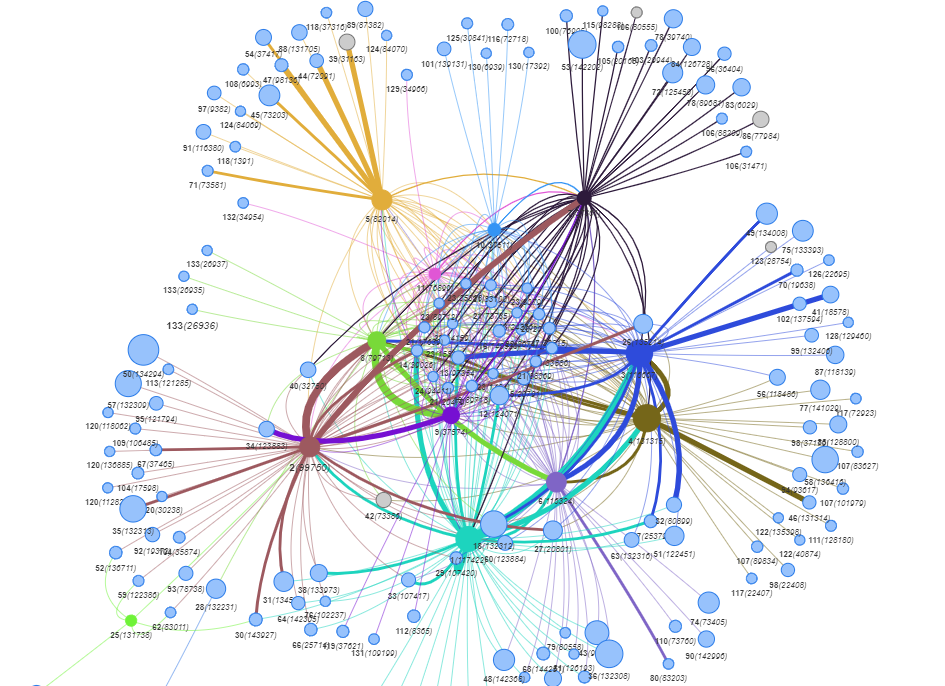
\includegraphics[width=\textwidth]{BandaLCDs1.png}
	\caption{Resultado de ejecución de PageRank para el caso real de robo de LCDs.} 
	\label{fig:BandaLCDs1}
\end{figure}
